\documentclass[12pt,a4paper]{article}
\input{library}
%Header
\fancyhead{} % clear all header fields
\fancyhead[L]{
 \begin{tabular}{rl}
    \begin{picture}(25,15)(0,0)
    \put(0,-8){\includegraphics[width=12mm, height=12mm]{pictures/hcmut.png}}
    %\put(0,-8){\epsfig{width=10mm,figure=hcmut.eps}}
   \end{picture}&
	%\includegraphics[width=8mm, height=8mm]{hcmut.png} & %
	\begin{tabular}{l}
		\textbf{\bf \ttfamily Trường Đại Học Bách Khoa - ĐHQG TP.Hồ Chí Minh}\\
		\textbf{\bf \ttfamily Khoa Cơ Khí - Bộ môn Cơ điện tử}
	\end{tabular} 	
 \end{tabular}
}
\fancyhead[R]{
	{\tiny \bf \quad} % Khoảng trắng nhỏ trong header bên phải
}

%Footer
\fancyfoot{} % clear all footer fields
\fancyfoot[L]{\scriptsize \ttfamily Kỹ thuật điều khiển tự động}
\fancyfoot[R]{\scriptsize \ttfamily Trang {\thepage}/9}
\renewcommand{\headrulewidth}{0.3pt}
\renewcommand{\footrulewidth}{0.3pt}
\begin{document}
    \begin{titlepage}   
    \begin{center}
        \vspace*{-2cm} 
        \large
        \textbf{ĐẠI HỌC QUỐC GIA THÀNH PHỐ HỒ CHÍ MINH \\
        TRƯỜNG ĐẠI HỌC BÁCH KHOA\\
        KHOA CƠ KHÍ\\
        BỘ MÔN CƠ ĐIỆN TỬ}\\
        \includegraphics[width=70mm, height=70mm]{pictures/hcmut.png} \\
        \rule{\linewidth}{0.5mm}\\
        \vspace{0.8cm}
        \Large
        \textbf{BÁO CÁO BÀI TẬP LỚN}\\
        \vspace*{0.5cm}
        \Huge
        \textbf{KỸ THUẬT \\ĐIỀU KHIỂN TỰ ĐỘNG}\\
        \vspace{0.5cm}
        \rule{\linewidth}{0.5mm}\\
        \vspace{0.8cm}
        \large
        \textbf{GVHD: THẦY PHẠM CÔNG BẰNG}\\
        \vspace{0.5cm}
        SINH VIÊN THỰC HIỆN:\\[0.3cm]
        \begin{tabular}{|>{\centering\arraybackslash}m{5cm}|>{\centering\arraybackslash}m{7cm}|>{\centering\arraybackslash}m{5cm}|}
            \hline
             \textbf{Họ và tên} & \textbf{MSSV} \\
            \hline
            Đào Trọng Chân & 2210305 \\
            \hline
            Võ Hữu Dư & 2210604 \\
            \hline
            Dương Quang Duy & 2210497 \\
            \hline
            Nguyễn Quốc Trung & 2213701 \\
            \hline
        \end{tabular}
    \end{center}
        
    \vfill
    \large
    \begin{center}
        TP.HCM, \today
    \end{center}
\end{titlepage}

    \begin{center}
    \section*{LỜI CẢM ƠN}
\end{center}
\hspace*{1cm}Chúng em xin gửi lời cảm ơn chân thành và sâu sắc đến thầy Phạm Công Bằng, người đã tận tình giảng dạy, hướng dẫn và truyền đạt cho chúng em những kiến thức quý báu trong môn học “Kỹ thuật điều khiển tự động”.
Nhờ sự nhiệt huyết và tận tâm của thầy, chúng em không chỉ hiểu rõ hơn về các nguyên lý điều khiển mà còn có cơ hội vận dụng kiến thức để thực hiện bài tập lớn với đề tài "Bàn xoay sử dụng relay". Đây thực sự là một trải nghiệm học tập quý giá giúp chúng em nâng cao kỹ năng thực hành, tư duy sáng tạo và khả năng làm việc nhóm.
Chúng em cũng biết ơn sự chỉ bảo tận tình của thầy trong quá trình thực hiện bài tập lớn. Những lời góp ý và hướng dẫn của thầy đã giúp chúng em vượt qua khó khăn, hoàn thiện sản phẩm và đạt được kết quả như mong đợi.
Một lần nữa, chúng em xin gửi lời cảm ơn sâu sắc đến thầy và kính chúc thầy luôn mạnh khỏe, hạnh phúc, thành công trong sự nghiệp giảng dạy và nghiên cứu.
\cleardoublepage
    \tableofcontents
    \cleardoublepage 
    \section{Các thành phần và sơ đồ đấu nối}
\subsection{Các thành phần}
\subsubsection{Relay trung gian}
\begin{itemize}
    \item \textbf{Cấu tạo relay trung gian:} Relay trung gian được cấu tạo gồm 2 bộ phận: Nam châm điện cùng hệ thống các tiếp điểm đóng ngắt 
    , được dùng rất nhiều trong ngành điện tử, điện công nghiệp \dots
    \begin{itemize}
        \item Nam châm điện: Được thiết kế gồm: lõi thép động, lõi thép tĩnh, cuộn dây
        (cuộn dây cường độ, cuộn điện áp hoặc cả 2). Lõi thép động được định vị bằng vít điều chỉnh, và găng bằng lò xo. 
        \item Mạch tiếp điểm. 
    \end{itemize}
    \item \textbf{Nguyên lý hoạt động:} Dòng điện chạy qua relay trung gian sẽ chạy qua cuộn dây bên trong và tạo ra một từ trường hút. Tác động lên đòn bẩy bên trong làm đóng hoặc mở các tiếp điểm điện. Trạng thái của relay được thay đổi, số tiếp điểm bị
    thay đổi 1 chiều hoặc nhiều chiều phụ thuộc vào thiết kế.
    \begin{figure}[H]
        \centering
        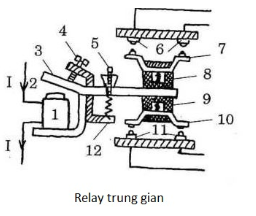
\includegraphics[width=0.5\textwidth]{pictures/NLHD_relay.png}
    \end{figure}
    \item Relay trung gian MY4N AC240/250, 14 chân, 5A (4PDT)
    \begin{figure}[H]
        \centering
        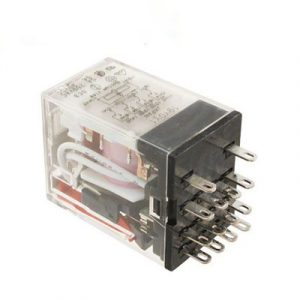
\includegraphics[width=0.5\textwidth]{pictures/Relay_4PDT.png}
    \end{figure}
    \item Relay trung gian MY2N AC240/250, 8 chân, 5A (DPDT)
    \begin{figure}[H]
        \centering
        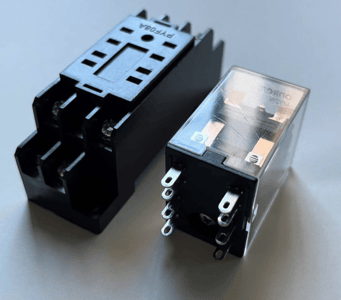
\includegraphics[width=0.5\textwidth]{pictures/Relay_DPDT.png}
    \end{figure}
\end{itemize}

\subsubsection{Module relay 4 kênh}
Module relay được sử dụng chung với cảm biến phát hiện kim loại. 
\begin{figure}[H]
    \centering
    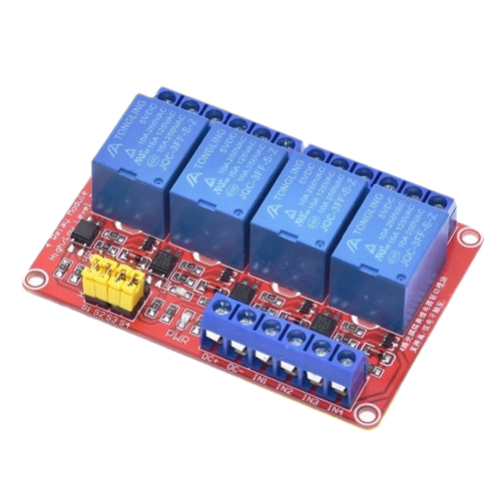
\includegraphics[width=0.5\textwidth]{pictures/Module_relay.png}
\end{figure}



\subsubsection{Cảm biến tiệm cận kim loại}
\begin{itemize}
    \item Cảm biến tiệm cận (Proximity Sensors). Còn có tên gọi khác là công tắc tiệm cận
    hay "PROX". Phản ứng khi có vật ở gần cảm biến.
    \item \textbf{Nguyên lý hoạt động:} Cảm biến tiệm cận NPN hoạt động dựa trên nguyên lý của 
    transitor NPN. Cấu tạo của cảm biến tiệm cận bao gồm 1 mạch phát hiện vật, mục đích để xử lí tín hiệu
    khi phát hiện vật gần cảm biến và chuyển đổi thành tín hiện điện cho mạch kế tiếp. Tiếp theo là 1 mạch ON/OFF NPN sử dụng tín hiệu
    điện từ mạch phát hiện vật để đóng ngắt transistor. Cuối cùng tín hiệu được xuất ra ngoài output (Output có thể là PLC, relay hoặc tải, \dots)
    \begin{figure}[H]
        \centering
        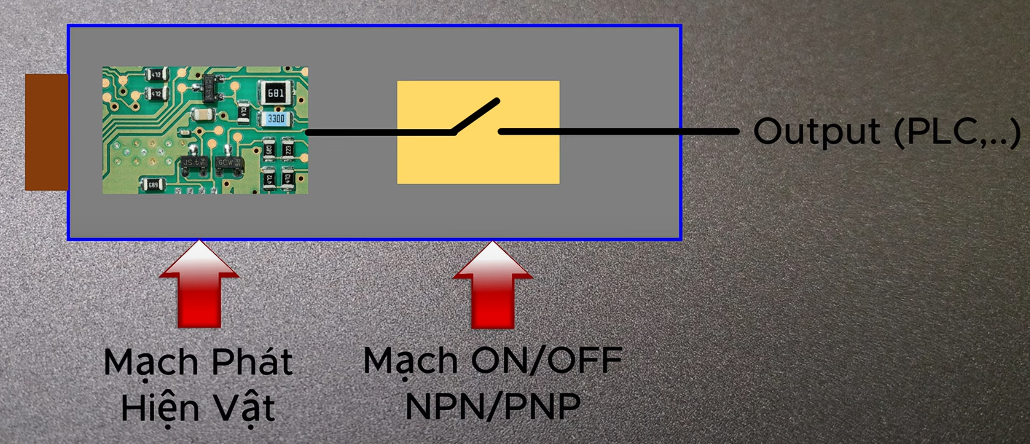
\includegraphics[width=0.7\textwidth]{pictures/structure_sensor.png}
    \end{figure}
    Cách đấu nối dây cho mạch sử dụng cảm biến tiệm cận kim loại NPN:
    \begin{figure}[H]
        \centering
        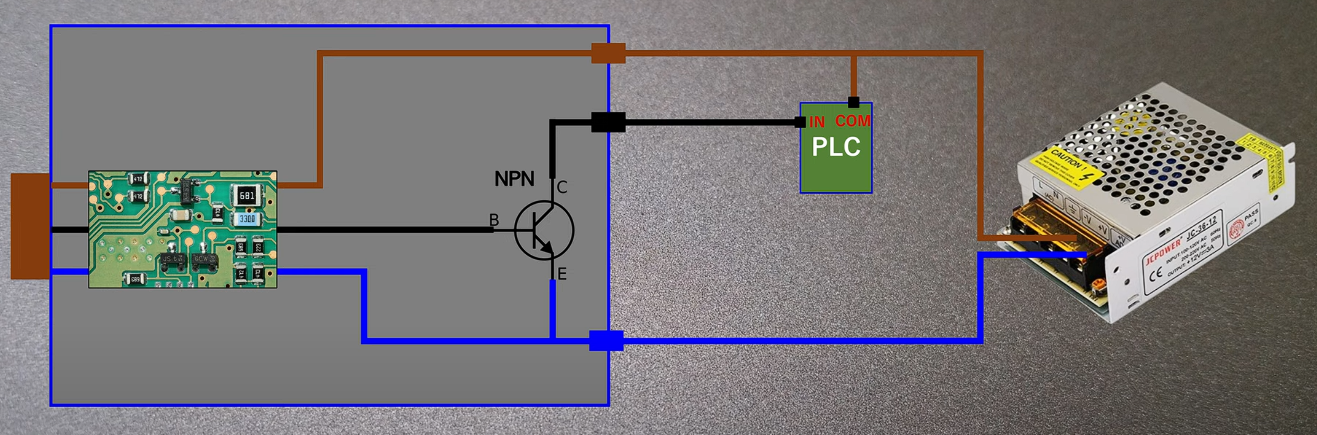
\includegraphics[width=1\textwidth]{pictures/mach_sensor.png}
    \end{figure}
    Trong trường hợp ở đây, chân tín hiệu của cảm biến sẽ được kết nối với module relay nhằm thực hiện nhiệm vụ như 1 công tắc trong mạch điều khiển
    ở các vị trí A1, B1, A2, B2.
\end{itemize}
Cảm biến phát hiện kim loại LJ12A3 loại NPN. 
\begin{figure}[H]
    \centering
    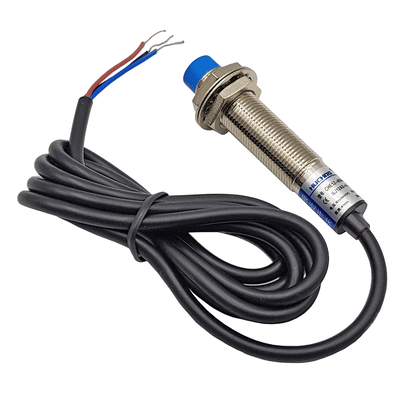
\includegraphics[width=0.5\textwidth]{pictures/Sensor.png}
\end{figure}
\cleardoublepage



\subsubsection{Động cơ}
Động cơ giảm tốc hộp số vuông góc JGY370 18RPM
\begin{figure}[H]
    \centering
    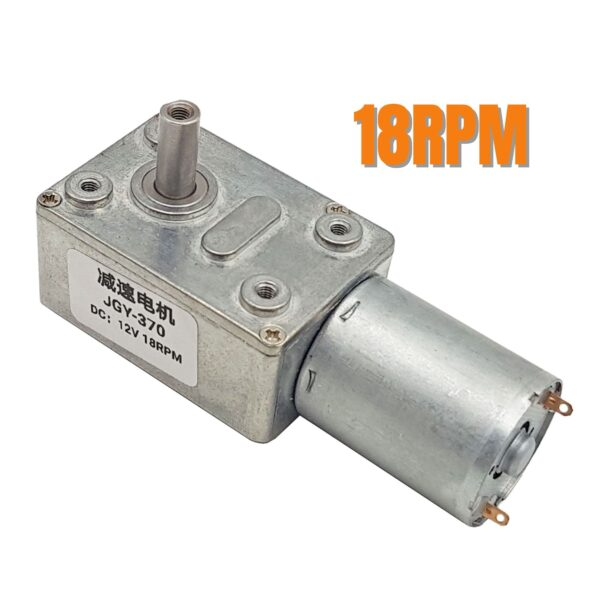
\includegraphics[width=0.5\textwidth]{pictures/motor.png}
\end{figure}
\subsection{Sơ đồ đấu nối}
\begin{figure}[H]
    \centering
    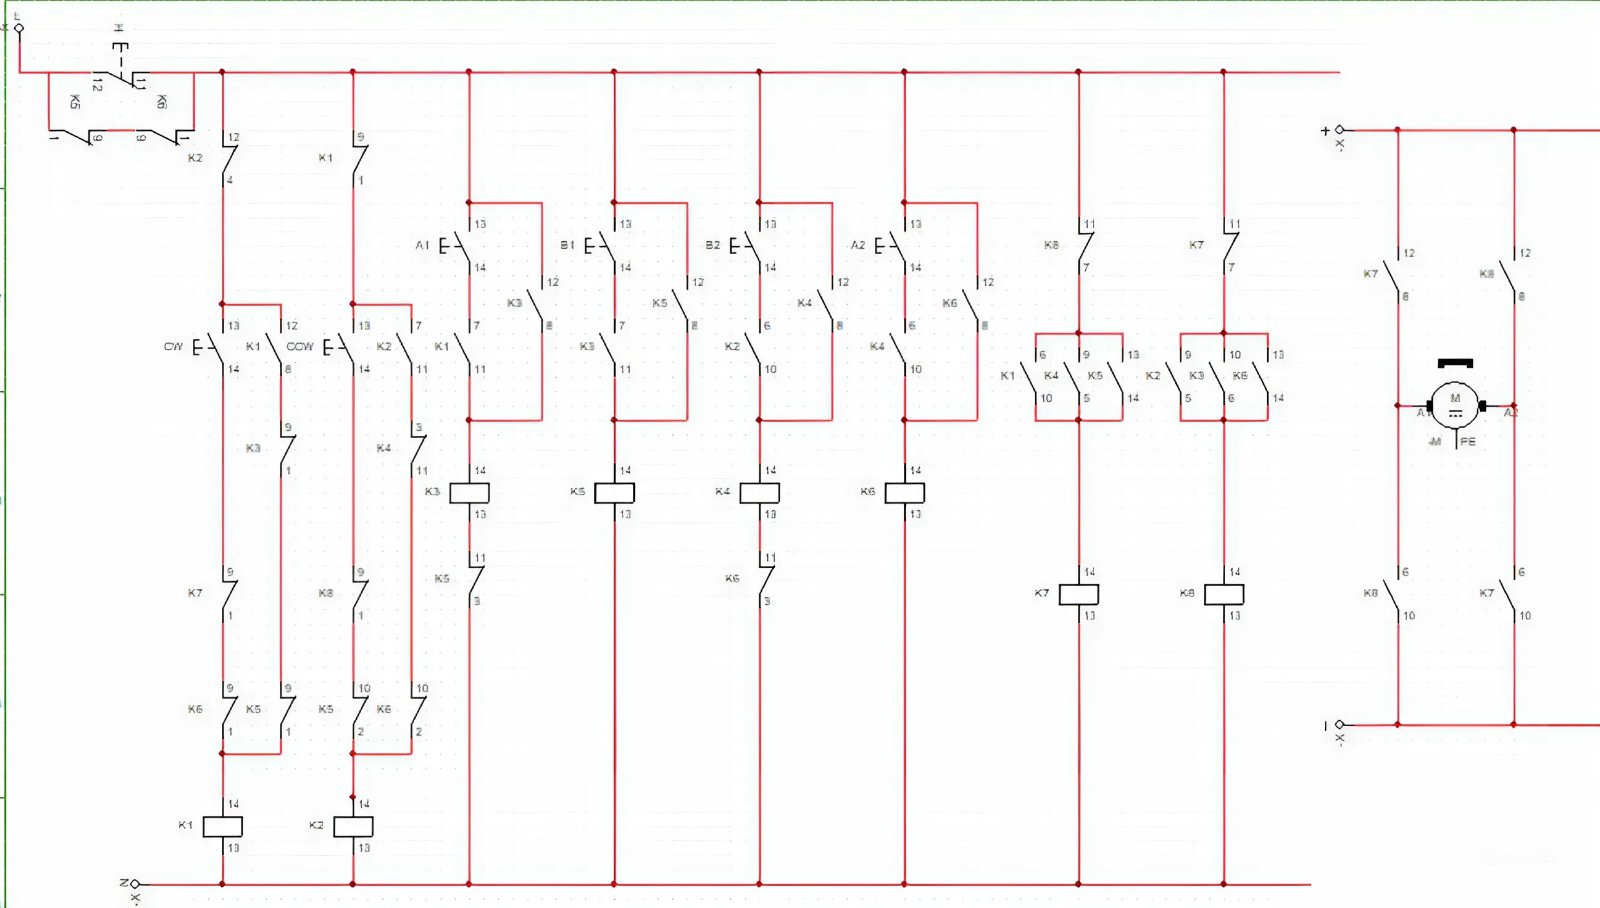
\includegraphics[width=1\textwidth]{pictures/connection.jpg}
\end{figure}
\cleardoublepage
    \section{Trình bày sơ đồ khối trong SFC}
Sơ đồ khối SFC  
\begin{figure}[H]
    \centering
    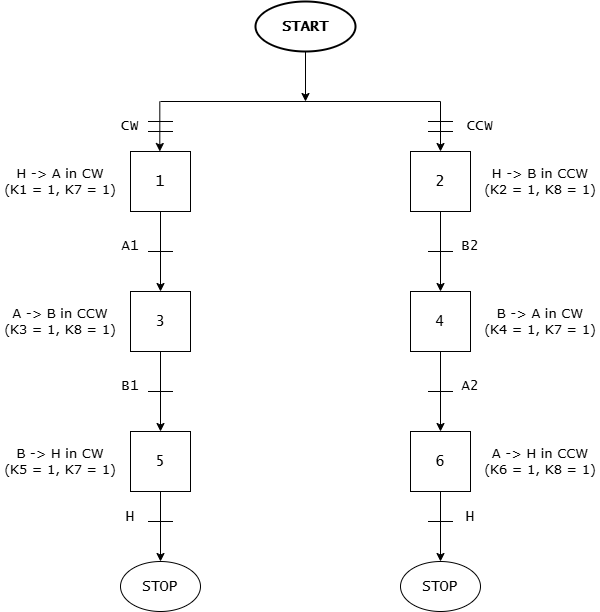
\includegraphics[width=0.9\textwidth]{pictures/SFC.png}
\end{figure}
Trong đó 2 nhánh lần lượt bắt đầu bằng CW, CCW thể hiện cho 2 nút bấm, 2 chế độ quay của bàn xoay.\\
Trong từng nhánh, các kí hiệu $Ki = 1 \,(i = 1, 2, \dots ,8)$ thể hiện trạng thái có điện của các cuộn dây $i$ tương ứng.
Trong đó $K7 = 1, \,K8 = 1$ lần lượt thể hiện cho chiều quay thuận và ngược chiều kim đồng hồ của động cơ.
\cleardoublepage
    \section{Triển khai mạch điều khiển và mạch động lực cho hệ thống}
\subsection{Mạch điều khiển}
\begin{figure}[H]
    \centering
    \includegraphics[width=0.8\textwidth]{pictures/control.png}
\end{figure}
\cleardoublepage
\subsection{Mạch động lực}
\begin{figure}[H]
    \centering
    \includegraphics[width=0.6\textwidth]{pictures/power.png}
\end{figure}
\subsection{Bảng trạng thái của chiều quay động cơ}
\begin{center}
\begin{tabular}{|c|c|c|c|c|c|c|c|c|c|c|}
    \hline  
    Trạng thái & K1 & K2 & K3 & K4 & K5 & K6 & K7 & K8 & Chiều quay\\
    \hline
    1 & 1 & 0 & 0 & 0 & 0 & 0 & 1 & 0 & CW\\
    \hline
    2 & 0 & 1 & 0 & 0 & 0 & 0 & 0 & 1 & CCW\\
    \hline
    3 & 0 & 0 & 1 & 0 & 0 & 0 & 0 & 1 & CCW\\
    \hline
    4 & 0 & 0 & 0 & 1 & 0 & 0 & 1 & 0 & CW\\
    \hline
    5 & 0 & 0 & 0 & 0 & 1 & 0 & 1 & 0 & CW\\
    \hline
    6 & 0 & 0 & 0 & 0 & 0 & 1 & 0 & 1 & CCW\\
    \hline
\end{tabular}
\end{center}
\subsection{Nguyên lý hoạt động}
\hspace*{0.5cm}Khi nhấn nút CW bàn sẽ xoay theo chiều kim đồng hồ (H -> A theo chiều kim đồng hồ, A -> B ngược chiều kim đồng hồ, B -> H theo chiều kim đồng hồ)\\

Còn khi nhấn nút CCW bàn sẽ xoay theo ngược chiều kim đồng hồ (H -> B ngược chiều kim đồng hồ, B -> A theo chiều kim đồng hồ, A -> H ngược chiều kim đồng hồ)\\

Vì 2 trường hợp tương ứng với 2 nút nhấn có nguyên lý hoạt động tương tự nhau nên ở đây ta xét ví dụ khi nhấn nút CW:
\begin{itemize}
    \item Khi nút CW được nhấn, cuộn coil K1 được kích, 2 tiếp điểm thường mở của K1 đóng lại, đồng thời tiếp điểm thường đóng của K1 mở ra ở nhánh có nút CCW để khóa trái 2 nút.
\end{itemize}
\begin{figure}[H]
    \centering
    \rotatebox{270}{\includegraphics[width=0.3\textwidth]{pictures/nhannut.png}}
\end{figure}
\begin{itemize}
    \item Đồng thời cặp tiếp điểm thường đóng K1 ở mạch động lực đóng lại làm cuộn coil K7 được kích, động cơ quay theo chiều kim đồng hồ.
\end{itemize}
\begin{figure}[H]
    \centering
    \includegraphics[width=0.5\textwidth]{pictures/kichK1.png}
\end{figure}
\begin{itemize}
    \item Cặp tiếp điểm K1 ở nhánh có cảm biến tại vị trí A đóng lại để khi có tín hiệu từ cảm biến, cuộn coil K3 sẽ được kích.
\end{itemize}
\begin{figure}[H]
    \centering
    \rotatebox{270}{\includegraphics[width=0.3\textwidth]{pictures/denA.png}}
\end{figure}
\begin{itemize}
    \item Khi có tín hiệu từ cảm biến ở vị trí A, cuộn coil K3 được kích, cặp tiếp điểm thường đóng ở nhánh có nút CW mở ra để cuộn coil K1 ngưng kích từ đó cuộn coil K7 cũng ngưng kích theo.
    \item Cặp tiếp điểm thường mở K3 ở mạch động lực đóng lại, cuộn coil K8 được kích động cơ quay ngược chiều kim đồng hồ. 
\end{itemize}
\begin{figure}[H]
    \centering
    \includegraphics[width=0.5\textwidth]{pictures/kichK3.png}
\end{figure}
\begin{itemize}
    \item Cặp tiếp điểm thường mở của K3 ở nhánh có cảm biến tại vị trí B đóng lại để khi có tín hiệu từ cảm biến, cuộn coil K5 sẽ được kích.
\end{itemize}
\begin{figure}[H]
    \centering
    \rotatebox{270}{\includegraphics[width=0.3\textwidth]{pictures/denB.png}}
\end{figure}
\begin{itemize}
    \item Khi có tín hiệu từ cảm biến ở vị trí B, cuộn coil K5 được kích, cặp tiếp điểm thường đóng ở nhánh có nút CW mở ra để cuộn coil K3 ngưng kích từ đó cuộn coil K8 cũng ngưng kích theo.
    \item Cặp tiếp điểm thường đóng K5 ở mạch động lực đóng lại, cuộn coil K7 được kích động cơ quay theo chiều kim đồng hồ.
\end{itemize}
\begin{figure}[H]
    \centering
    \includegraphics[width=0.5\textwidth]{pictures/kichK5.png}
\end{figure}
\begin{itemize}
    \item Một cặp tiếp điểm thường đóng của K5 ở nhánh có cảm biến tại vị trí H mở ra để khi có tín hiệu từ cảm biến, toàn bộ mạch điện sẽ được ngắt điện và trở về trạng thái ban đầu, kết thúc 1 chu kỳ.
\end{itemize}
\begin{figure}[H]
    \centering
    \includegraphics[width=0.5\textwidth]{pictures/denH.png}
\end{figure}
\begin{itemize}
    \item Khi 1 trong 2 nút được nhấn, hệ thống tiếp tục hoạt động theo nguyên lý trên.
\end{itemize}
\cleardoublepage
    \input{d.tex}
\end{document}